\documentclass[]{tufte-handout}

% ams
\usepackage{amssymb,amsmath}

\usepackage{ifxetex,ifluatex}
\usepackage{fixltx2e} % provides \textsubscript
\ifnum 0\ifxetex 1\fi\ifluatex 1\fi=0 % if pdftex
  \usepackage[T1]{fontenc}
  \usepackage[utf8]{inputenc}
\else % if luatex or xelatex
  \makeatletter
  \@ifpackageloaded{fontspec}{}{\usepackage{fontspec}}
  \makeatother
  \defaultfontfeatures{Ligatures=TeX,Scale=MatchLowercase}
  \makeatletter
  \@ifpackageloaded{soul}{
     \renewcommand\allcapsspacing[1]{{\addfontfeature{LetterSpace=15}#1}}
     \renewcommand\smallcapsspacing[1]{{\addfontfeature{LetterSpace=10}#1}}
   }{}
  \makeatother

\fi

% graphix
\usepackage{graphicx}
\setkeys{Gin}{width=\linewidth,totalheight=\textheight,keepaspectratio}

% booktabs
\usepackage{booktabs}

% url
\usepackage{url}

% hyperref
\usepackage{hyperref}

% units.
\usepackage{units}


\setcounter{secnumdepth}{-1}

% citations
\usepackage{natbib}
\bibliographystyle{plainnat}


% pandoc syntax highlighting
\usepackage{color}
\usepackage{fancyvrb}
\newcommand{\VerbBar}{|}
\newcommand{\VERB}{\Verb[commandchars=\\\{\}]}
\DefineVerbatimEnvironment{Highlighting}{Verbatim}{commandchars=\\\{\}}
% Add ',fontsize=\small' for more characters per line
\newenvironment{Shaded}{}{}
\newcommand{\AlertTok}[1]{\textcolor[rgb]{1.00,0.00,0.00}{\textbf{#1}}}
\newcommand{\AnnotationTok}[1]{\textcolor[rgb]{0.38,0.63,0.69}{\textbf{\textit{#1}}}}
\newcommand{\AttributeTok}[1]{\textcolor[rgb]{0.49,0.56,0.16}{#1}}
\newcommand{\BaseNTok}[1]{\textcolor[rgb]{0.25,0.63,0.44}{#1}}
\newcommand{\BuiltInTok}[1]{\textcolor[rgb]{0.00,0.50,0.00}{#1}}
\newcommand{\CharTok}[1]{\textcolor[rgb]{0.25,0.44,0.63}{#1}}
\newcommand{\CommentTok}[1]{\textcolor[rgb]{0.38,0.63,0.69}{\textit{#1}}}
\newcommand{\CommentVarTok}[1]{\textcolor[rgb]{0.38,0.63,0.69}{\textbf{\textit{#1}}}}
\newcommand{\ConstantTok}[1]{\textcolor[rgb]{0.53,0.00,0.00}{#1}}
\newcommand{\ControlFlowTok}[1]{\textcolor[rgb]{0.00,0.44,0.13}{\textbf{#1}}}
\newcommand{\DataTypeTok}[1]{\textcolor[rgb]{0.56,0.13,0.00}{#1}}
\newcommand{\DecValTok}[1]{\textcolor[rgb]{0.25,0.63,0.44}{#1}}
\newcommand{\DocumentationTok}[1]{\textcolor[rgb]{0.73,0.13,0.13}{\textit{#1}}}
\newcommand{\ErrorTok}[1]{\textcolor[rgb]{1.00,0.00,0.00}{\textbf{#1}}}
\newcommand{\ExtensionTok}[1]{#1}
\newcommand{\FloatTok}[1]{\textcolor[rgb]{0.25,0.63,0.44}{#1}}
\newcommand{\FunctionTok}[1]{\textcolor[rgb]{0.02,0.16,0.49}{#1}}
\newcommand{\ImportTok}[1]{\textcolor[rgb]{0.00,0.50,0.00}{\textbf{#1}}}
\newcommand{\InformationTok}[1]{\textcolor[rgb]{0.38,0.63,0.69}{\textbf{\textit{#1}}}}
\newcommand{\KeywordTok}[1]{\textcolor[rgb]{0.00,0.44,0.13}{\textbf{#1}}}
\newcommand{\NormalTok}[1]{#1}
\newcommand{\OperatorTok}[1]{\textcolor[rgb]{0.40,0.40,0.40}{#1}}
\newcommand{\OtherTok}[1]{\textcolor[rgb]{0.00,0.44,0.13}{#1}}
\newcommand{\PreprocessorTok}[1]{\textcolor[rgb]{0.74,0.48,0.00}{#1}}
\newcommand{\RegionMarkerTok}[1]{#1}
\newcommand{\SpecialCharTok}[1]{\textcolor[rgb]{0.25,0.44,0.63}{#1}}
\newcommand{\SpecialStringTok}[1]{\textcolor[rgb]{0.73,0.40,0.53}{#1}}
\newcommand{\StringTok}[1]{\textcolor[rgb]{0.25,0.44,0.63}{#1}}
\newcommand{\VariableTok}[1]{\textcolor[rgb]{0.10,0.09,0.49}{#1}}
\newcommand{\VerbatimStringTok}[1]{\textcolor[rgb]{0.25,0.44,0.63}{#1}}
\newcommand{\WarningTok}[1]{\textcolor[rgb]{0.38,0.63,0.69}{\textbf{\textit{#1}}}}

% table with pandoc
\usepackage{longtable,booktabs,array}
\usepackage{calc} % for calculating minipage widths
% Correct order of tables after \paragraph or \subparagraph
\usepackage{etoolbox}
\makeatletter
\patchcmd\longtable{\par}{\if@noskipsec\mbox{}\fi\par}{}{}
\makeatother
% Allow footnotes in longtable head/foot
\IfFileExists{footnotehyper.sty}{\usepackage{footnotehyper}}{\usepackage{footnote}}
\makesavenoteenv{longtable}

% multiplecol
\usepackage{multicol}

% strikeout
\usepackage[normalem]{ulem}

% morefloats
\usepackage{morefloats}


% tightlist macro required by pandoc >= 1.14
\providecommand{\tightlist}{%
  \setlength{\itemsep}{0pt}\setlength{\parskip}{0pt}}

% title / author / date
\title{Lab 07 - Smokers in Whickham}
\author{Dina Alarcon}
\date{}


\begin{document}

\maketitle




\subsection{Introduction}\label{introduction}

A study conducted in Whickham, England recorded participants' age,
smoking status at baseline, and then 20 years later recorded their
health outcome. In this lab we analyze the relationships between these
variables, first two at a time, and then controlling for a third
variable.

\textbf{You might be surprised by what you find!} This lab demonstrates
an important statistical phenomenon called \textbf{Simpson's paradox},
where a trend that appears in different groups of data disappears or
reverses when the groups are combined. Understanding this paradox is
crucial for correctly interpreting data and avoiding misleading
conclusions.

\textbf{Estimated time:} 60-90 minutes

\subsection{Learning Goals}\label{learning-goals}

By the end of this lab, you will be able to:

\begin{itemize}
\tightlist
\item
  Distinguish between observational studies and experiments
\item
  Visualize relationships between categorical variables
\item
  Calculate and interpret conditional probabilities
\item
  Create categorical variables from continuous variables using
  \texttt{case\_when()}
\item
  Use faceting to explore three-way relationships
\item
  Identify and explain Simpson's paradox
\item
  Understand the role of confounding variables
\end{itemize}

\subsection{Prerequisites}\label{prerequisites}

Before you begin, make sure you have:

\begin{itemize}
\tightlist
\item
  ✅ Completed Labs 01-06
\item
  ✅ Watched lectures on categorical data and conditional probability
\item
  ✅ Understand bar plots and mosaic plots
\item
  ✅ Forked the lab-instructions repository
\end{itemize}

\begin{center}\rule{0.5\linewidth}{0.5pt}\end{center}

\section{Getting Started}\label{getting-started}

Navigate to your forked \texttt{lab-instructions} repository in
JupyterHub, open the \texttt{Lab07} folder, and open the R Markdown
document \texttt{lab-07.Rmd}.

\subsection{Verify Your Setup}\label{verify-your-setup}

Before proceeding:

Step 1. Open \texttt{lab-07.Rmd} in RStudio

Step 2. Check that the Git pane shows YOUR username (not the course
organization)

Step 3. Click \textbf{Knit} to make sure the document compiles

\subsection{Warm Up}\label{warm-up}

Before we introduce the data, let's warm up with some simple exercises.

\textbf{Step 1:} Update the YAML, changing the author name to your name.

\textbf{Step 2:} Knit the document.

\textbf{Step 3:} Commit your changes with message ``Updated author
name''.

\textbf{Step 4:} Push to GitHub and verify the changes are visible in
your repo.

🧶 ✅ ⬆️ \textbf{Knit, commit with message ``Completed warm up'', and
push your changes.}

\begin{center}\rule{0.5\linewidth}{0.5pt}\end{center}

\subsection{Packages}\label{packages}

We'll use the \textbf{tidyverse} package for much of the data wrangling
and visualisation and the data lives in the \textbf{mosaicData} package.
These packages are already installed for you. You can load them by
running the following in your Console:

\begin{Shaded}
\begin{Highlighting}[]
\FunctionTok{library}\NormalTok{(tidyverse) }
\FunctionTok{library}\NormalTok{(mosaicData) }
\end{Highlighting}
\end{Shaded}

\subsection{Data}\label{data}

The dataset we'll use is called \texttt{Whickham} from the
\textbf{mosaicData} package. You can find out more about the dataset by
inspecting its documentation, which you can access by running
\texttt{?Whickham} in the Console or using the Help menu in RStudio to
search for \texttt{Whickham}.

\textbf{✓ Checkpoint:} Run \texttt{glimpse(Whickham)} in your Console to
verify the data loaded correctly.

\begin{center}\rule{0.5\linewidth}{0.5pt}\end{center}

\section{Exercises}\label{exercises}

\subsection{Understanding the Study}\label{understanding-the-study}

\subsection{Exercise 1}\label{exercise-1}

What type of study do you think these data come from: observational or
experiment? Why?

\textbf{Definitions to help you decide:}

\begin{itemize}
\tightlist
\item
  \textbf{Observational study:} Researchers observe and measure
  variables but don't intervene or assign treatments
\item
  \textbf{Experiment:} Researchers actively assign
  treatments/interventions to participants
\end{itemize}

\textbf{Your answer:}

This is an observational study because researchers recorded
participants' smoking status and followed their health outcomes after 20
years. They did not assign participants to smoke or not smoke.

\begin{center}\rule{0.5\linewidth}{0.5pt}\end{center}

\subsection{Exercise 2}\label{exercise-2}

How many observations are in this dataset? What does each observation
represent?

\textbf{Hint:} Use inline code with \texttt{nrow()} to report the number
of observations.

\textbf{Your answer:}

The dataset has 1314 observations. Each observation represents one
participant, including their age, smoking status at baseline, and
whether they were alive or dead 20 years later.

🧶 ✅ ⬆️ \textbf{Knit, commit with message ``Completed Exercises 1-2'',
and push your changes.}

\begin{center}\rule{0.5\linewidth}{0.5pt}\end{center}

\subsection{Exploring the Variables}\label{exploring-the-variables}

\subsection{Exercise 3}\label{exercise-3}

How many variables are in this dataset? What type of variable is each?
Display each variable using an appropriate visualization.

\textbf{Part A: Count and classify the variables}

Run \texttt{glimpse(Whickham)} in your Console to see the variables.

\textbf{Number of variables:} \_\_\_\_\_

\textbf{Variable types:}

\begin{longtable}[]{@{}lll@{}}
\toprule\noalign{}
Variable & Type (categorical/numerical) & More specific type \\
\midrule\noalign{}
\endhead
\bottomrule\noalign{}
\endlastfoot
outcome & categorical & Binary, nominal \\
smoker & categorical & Binary, nominal \\
age & numerical & whole years \\
\end{longtable}

\textbf{Part B: Create visualizations}

Create appropriate visualizations for each variable.

\textbf{For categorical variables (outcome and smoker):}

\begin{Shaded}
\begin{Highlighting}[]
\CommentTok{\# Remember to change eval=FALSE to eval=TRUE!}

\CommentTok{\# Outcome variable}
\FunctionTok{ggplot}\NormalTok{(Whickham, }\FunctionTok{aes}\NormalTok{(}\AttributeTok{x =}\NormalTok{ outcome)) }\SpecialCharTok{+}
  \FunctionTok{geom\_bar}\NormalTok{(}\AttributeTok{fill =} \StringTok{"seagreen"}\NormalTok{) }\SpecialCharTok{+}
  \FunctionTok{labs}\NormalTok{(}
    \AttributeTok{title =} \StringTok{"Participants\textquotesingle{} Outcomes After 20 Years"}\NormalTok{,}
    \AttributeTok{x =} \StringTok{"Outcome"}\NormalTok{,}
    \AttributeTok{y =} \StringTok{"Number of Participants"}
\NormalTok{  )}
\end{Highlighting}
\end{Shaded}

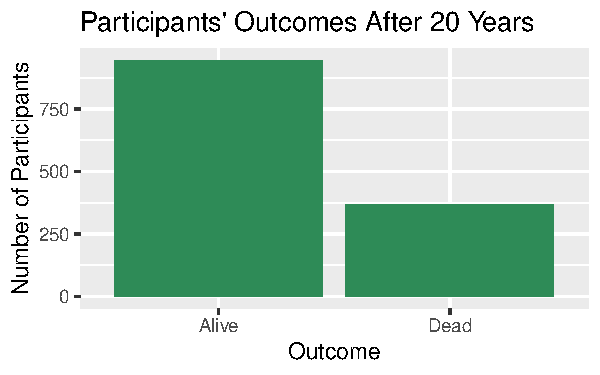
\includegraphics{lab-07-simpsons-paradox_files/figure-latex/visualize-categorical-1}

\begin{Shaded}
\begin{Highlighting}[]
\FunctionTok{ggplot}\NormalTok{(Whickham, }\FunctionTok{aes}\NormalTok{(}\AttributeTok{x =}\NormalTok{ smoker)) }\SpecialCharTok{+}
  \FunctionTok{geom\_bar}\NormalTok{(}\AttributeTok{fill =} \StringTok{"deeppink3"}\NormalTok{) }\SpecialCharTok{+}
  \FunctionTok{labs}\NormalTok{(}
    \AttributeTok{title =} \StringTok{"Participants\textquotesingle{} Smoking Status at Baseline"}\NormalTok{,}
    \AttributeTok{x =} \StringTok{"Smoker"}\NormalTok{,}
    \AttributeTok{y =} \StringTok{"Number of Participants"}
\NormalTok{  )}
\end{Highlighting}
\end{Shaded}

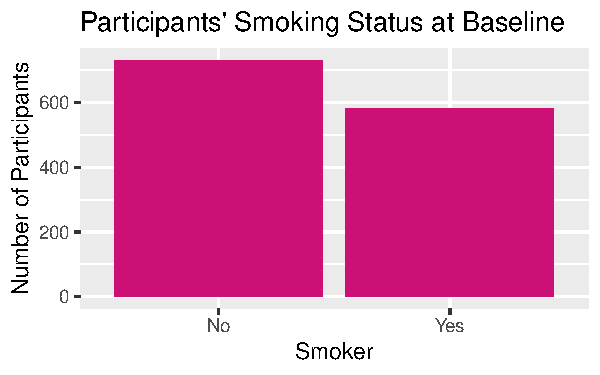
\includegraphics{lab-07-simpsons-paradox_files/figure-latex/visualize-categorical-2}

\textbf{For numerical variable (age):}

\begin{Shaded}
\begin{Highlighting}[]
\CommentTok{\# Remember to change eval=FALSE to eval=TRUE!}
\FunctionTok{ggplot}\NormalTok{(Whickham, }\FunctionTok{aes}\NormalTok{(}\AttributeTok{x =}\NormalTok{ age)) }\SpecialCharTok{+}
  \FunctionTok{geom\_histogram}\NormalTok{(}
    \AttributeTok{binwidth =} \DecValTok{5}\NormalTok{,}
    \AttributeTok{fill =} \StringTok{"plum"}\NormalTok{,}
    \AttributeTok{color =} \StringTok{"white"}
\NormalTok{  ) }\SpecialCharTok{+}
  \FunctionTok{labs}\NormalTok{(}
    \AttributeTok{title =} \StringTok{"Participants\textquotesingle{} Ages at Baseline"}\NormalTok{,}
    \AttributeTok{x =} \StringTok{"Age (years)"}\NormalTok{,}
    \AttributeTok{y =} \StringTok{"Number of Participants"}
\NormalTok{  )}
\end{Highlighting}
\end{Shaded}

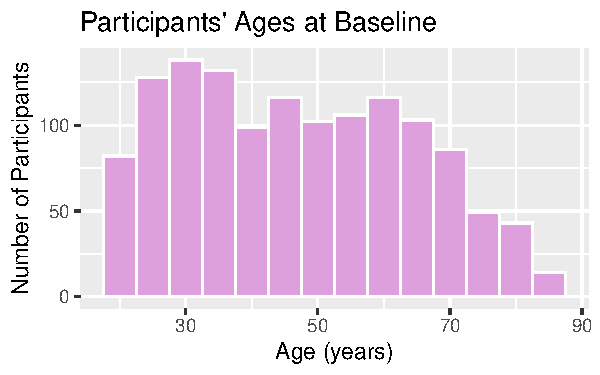
\includegraphics{lab-07-simpsons-paradox_files/figure-latex/visualize-age-1}

\textbf{Hint:} Try a binwidth of 5 or 10 for age.

\begin{center}\rule{0.5\linewidth}{0.5pt}\end{center}

\subsection{Making Predictions}\label{making-predictions}

\subsection{Exercise 4}\label{exercise-4}

What would you expect the relationship between smoking status and health
outcome to be?

\textbf{Think about it:} If we compare smokers to non-smokers after 20
years, what difference would you expect to see in their health outcomes?

\textbf{Your prediction:}

I would expect that smokers would have a higher proportion of deaths and
a lower proportion of survivors after 20 years compared with
non-smokers.

🧶 ✅ ⬆️ \textbf{Knit, commit with message ``Completed Exercises 3-4'',
and push your changes.}

\begin{center}\rule{0.5\linewidth}{0.5pt}\end{center}

\subsection{Examining the
Relationship}\label{examining-the-relationship}

\subsection{Exercise 5}\label{exercise-5}

Create a visualization depicting the relationship between smoking status
and health outcome. Briefly describe the relationship, and evaluate
whether this meets your expectations. Additionally, calculate the
relevant conditional probabilities to help your narrative.

\textbf{Part A: Create a visualization}

\begin{Shaded}
\begin{Highlighting}[]
\CommentTok{\# Remember to change eval=FALSE to eval=TRUE!}
\FunctionTok{ggplot}\NormalTok{(Whickham, }\FunctionTok{aes}\NormalTok{(}\AttributeTok{x =}\NormalTok{ smoker, }\AttributeTok{fill =}\NormalTok{ outcome)) }\SpecialCharTok{+}
  \FunctionTok{geom\_bar}\NormalTok{(}\AttributeTok{position =} \StringTok{"fill"}\NormalTok{) }\SpecialCharTok{+}
  \FunctionTok{scale\_fill\_manual}\NormalTok{(}
    \AttributeTok{values =} \FunctionTok{c}\NormalTok{(}\StringTok{"Alive"} \OtherTok{=} \StringTok{"plum"}\NormalTok{, }\StringTok{"Dead"} \OtherTok{=} \StringTok{"darkcyan"}\NormalTok{)}
\NormalTok{  ) }\SpecialCharTok{+}
  \FunctionTok{labs}\NormalTok{(}
    \AttributeTok{title =} \StringTok{"Health Outcomes After 20 Years by Smoking Status"}\NormalTok{,}
    \AttributeTok{x =} \StringTok{"Smoker at Baseline"}\NormalTok{,}
    \AttributeTok{y =} \StringTok{"Proportion of Participants"}\NormalTok{,}
    \AttributeTok{fill =} \StringTok{"Outcome"}
\NormalTok{  )}
\end{Highlighting}
\end{Shaded}

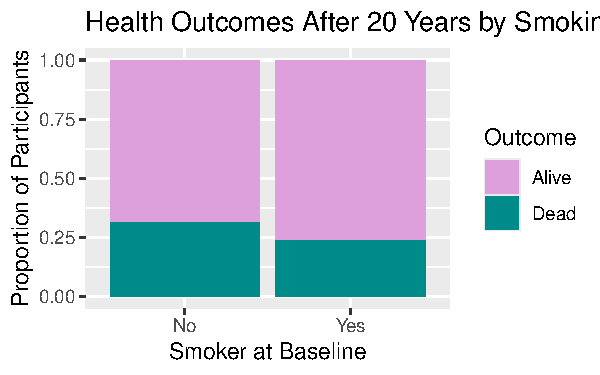
\includegraphics{lab-07-simpsons-paradox_files/figure-latex/smoker-outcome-viz-1}

\textbf{Hints:}

\begin{itemize}
\tightlist
\item
  Put \texttt{smoker} on the x-axis and fill by \texttt{outcome}
\item
  Try \texttt{position\ =\ "fill"} to show proportions, or
  \texttt{position\ =\ "dodge"} to show counts side-by-side
\end{itemize}

\textbf{Part B: Calculate counts}

Here is some code to get you started:

\begin{Shaded}
\begin{Highlighting}[]
\NormalTok{Whickham }\SpecialCharTok{\%\textgreater{}\%}
  \FunctionTok{count}\NormalTok{(smoker, outcome)}
\end{Highlighting}
\end{Shaded}

\begin{verbatim}
##   smoker outcome   n
## 1     No   Alive 502
## 2     No    Dead 230
## 3    Yes   Alive 443
## 4    Yes    Dead 139
\end{verbatim}

\textbf{What this shows:} The number of people in each combination of
smoking status and outcome.

\textbf{Part C: Calculate conditional probabilities}

Calculate the probability of being alive given smoking status.

\begin{Shaded}
\begin{Highlighting}[]
\CommentTok{\# Remember to change eval=FALSE to eval=TRUE!}
\NormalTok{Whickham }\SpecialCharTok{\%\textgreater{}\%}
  \FunctionTok{count}\NormalTok{(smoker, outcome) }\SpecialCharTok{\%\textgreater{}\%}
  \FunctionTok{group\_by}\NormalTok{(smoker) }\SpecialCharTok{\%\textgreater{}\%}
  \FunctionTok{mutate}\NormalTok{(}\AttributeTok{probability =}\NormalTok{ n }\SpecialCharTok{/} \FunctionTok{sum}\NormalTok{(n)) }\SpecialCharTok{\%\textgreater{}\%}
  \FunctionTok{ungroup}\NormalTok{()}
\end{Highlighting}
\end{Shaded}

\begin{verbatim}
## # A tibble: 4 x 4
##   smoker outcome     n probability
##   <fct>  <fct>   <int>       <dbl>
## 1 No     Alive     502       0.686
## 2 No     Dead      230       0.314
## 3 Yes    Alive     443       0.761
## 4 Yes    Dead      139       0.239
\end{verbatim}

\textbf{Interpret the results:}

\begin{itemize}
\tightlist
\item
  Proportion of smokers who are alive after 20 years:0.7612 (76.1\%)
\item
  Proportion of non-smokers who are alive after 20 years: 0.6858
  (68.6\%)
\end{itemize}

\textbf{Does this meet your expectations? What do you notice?} This does
not meet my expectations. In the combined data, smokers had a higher
survival proportion than non-smokers. Other factors, such as age, may
explain this unexpected pattern.

🧶 ✅ ⬆️ \textbf{Knit, commit with message ``Completed Exercise 5'', and
push your changes.}

\begin{center}\rule{0.5\linewidth}{0.5pt}\end{center}

\subsection{Adding a Third Variable}\label{adding-a-third-variable}

\subsection{Exercise 6}\label{exercise-6}

Create a new variable called \texttt{age\_cat} using the following
scheme:

\begin{itemize}
\tightlist
\item
  age ≤ 44 → ``18-44''
\item
  age \textgreater{} 44 and age ≤ 64 → ``45-64''
\item
  age \textgreater{} 64 → ``65+''
\end{itemize}

\textbf{Use \texttt{case\_when()} to create the categorical variable:}

\begin{Shaded}
\begin{Highlighting}[]
\CommentTok{\# Remember to change eval=FALSE to eval=TRUE!}
\NormalTok{Whickham \%}
  \FunctionTok{mutate}\NormalTok{(}\AttributeTok{age\_cat =} \FunctionTok{case\_when}\NormalTok{(}
\NormalTok{    age }\SpecialCharTok{\textless{}=}\NormalTok{ \_\_\_ }\SpecialCharTok{\textasciitilde{}} \StringTok{"18{-}44"}\NormalTok{,}
\NormalTok{    age }\SpecialCharTok{\textgreater{}}\NormalTok{ \_\_\_ }\SpecialCharTok{\&}\NormalTok{ age }\SpecialCharTok{\textless{}=}\NormalTok{ \_\_\_ }\SpecialCharTok{\textasciitilde{}} \StringTok{"45{-}64"}\NormalTok{,}
\NormalTok{    age }\SpecialCharTok{\textgreater{}}\NormalTok{ \_\_\_ }\SpecialCharTok{\textasciitilde{}} \StringTok{"65+"}
\NormalTok{  ))}
\end{Highlighting}
\end{Shaded}

\textbf{What this code does:}

\begin{itemize}
\tightlist
\item
  Takes the \texttt{Whickham} dataset
\item
  Uses \texttt{mutate()} to create a new variable called
  \texttt{age\_cat}
\item
  \texttt{case\_when()} checks each condition in order and assigns the
  corresponding category
\item
  Saves the result back to \texttt{Whickham} using \texttt{\textless{}-}
\end{itemize}

\textbf{Verify it worked:}

\begin{Shaded}
\begin{Highlighting}[]
\CommentTok{\# Remember to change eval=FALSE to eval=TRUE!}
\NormalTok{Whickham }\SpecialCharTok{\%\textgreater{}\%}
  \FunctionTok{count}\NormalTok{(age\_cat)}
\end{Highlighting}
\end{Shaded}

\textbf{How many people are in each age category?}

\begin{itemize}
\tightlist
\item
  18-44: \_\_\_\_\_
\item
  45-64: \_\_\_\_\_
\item
  65+: \_\_\_\_\_
\end{itemize}

\begin{center}\rule{0.5\linewidth}{0.5pt}\end{center}

\subsection{The Big Reveal: Simpson's
Paradox}\label{the-big-reveal-simpsons-paradox}

\subsection{Exercise 7}\label{exercise-7}

Re-create the visualization depicting the relationship between smoking
status and health outcome, faceted by \texttt{age\_cat}. What changed?
What might explain this change?

\textbf{Part A: Create the faceted visualization}

\begin{Shaded}
\begin{Highlighting}[]
\CommentTok{\# Remember to change eval=FALSE to eval=TRUE!}
\FunctionTok{ggplot}\NormalTok{(}\AttributeTok{data =}\NormalTok{ Whickham, }\FunctionTok{aes}\NormalTok{(}\AttributeTok{x =}\NormalTok{ \_\_\_, }\AttributeTok{fill =}\NormalTok{ \_\_\_)) }\SpecialCharTok{+}
  \FunctionTok{geom\_bar}\NormalTok{(}\AttributeTok{position =} \StringTok{"\_\_\_"}\NormalTok{) }\SpecialCharTok{+}
  \FunctionTok{facet\_wrap}\NormalTok{(}\SpecialCharTok{\textasciitilde{}}\NormalTok{\_\_\_) }\SpecialCharTok{+}
  \FunctionTok{labs}\NormalTok{(}
    \AttributeTok{title =} \StringTok{"\_\_\_"}\NormalTok{,}
    \AttributeTok{x =} \StringTok{"\_\_\_"}\NormalTok{,}
    \AttributeTok{y =} \StringTok{"\_\_\_"}\NormalTok{,}
    \AttributeTok{fill =} \StringTok{"\_\_\_"}
\NormalTok{  )}
\end{Highlighting}
\end{Shaded}

\textbf{Hint:} Use the same aesthetics as Exercise 5, but add
\texttt{facet\_wrap(\textasciitilde{}age\_cat)}

\textbf{Part B: Examine the three-way contingency table}

Extend the contingency table from earlier by breaking it down by age
category:

\begin{Shaded}
\begin{Highlighting}[]
\CommentTok{\# Remember to change eval=FALSE to eval=TRUE!}
\NormalTok{Whickham }\SpecialCharTok{\%\textgreater{}\%}
  \FunctionTok{count}\NormalTok{(smoker, age\_cat, outcome)}
\end{Highlighting}
\end{Shaded}

\textbf{Calculate proportions within each age group:}

\begin{Shaded}
\begin{Highlighting}[]
\CommentTok{\# Remember to change eval=FALSE to eval=TRUE!}
\NormalTok{Whickham }\SpecialCharTok{\%\textgreater{}\%}
  \FunctionTok{count}\NormalTok{(smoker, age\_cat, outcome) }\SpecialCharTok{\%\textgreater{}\%}
  \FunctionTok{group\_by}\NormalTok{(\_\_\_, \_\_\_) }\SpecialCharTok{\%\textgreater{}\%}
  \FunctionTok{mutate}\NormalTok{(}\AttributeTok{proportion =}\NormalTok{ n }\SpecialCharTok{/} \FunctionTok{sum}\NormalTok{(n))}
\end{Highlighting}
\end{Shaded}

\textbf{Part C: Interpret the results}

\textbf{What changed when you added age\_cat?}

\textbf{Compare the relationship between smoking and outcome:}

\textbf{Overall (from Exercise 5):} Smokers appeared to have
\_\_\_\_\_\_\_\_\_\_\_\_\_\_\_\_\_\_\_\_\_ survival

\textbf{Within each age group (from Exercise 7):} Smokers appear to have

\textbf{What might explain this change?}

Consider:

\begin{itemize}
\tightlist
\item
  Which age groups have more smokers?
\item
  Which age groups have higher survival rates overall?
\item
  How might age affect both smoking status and survival?
\end{itemize}

\textbf{Your explanation:}

🧶 ✅ ⬆️ \textbf{Knit, commit with message ``Completed Exercises 6-7'',
and push your changes.}

\begin{center}\rule{0.5\linewidth}{0.5pt}\end{center}

\subsection{Understanding Simpson's
Paradox}\label{understanding-simpsons-paradox}

\textbf{What you just discovered is called Simpson's Paradox!}

\begin{marginfigure}
Simpson's paradox was first described by Edward Simpson in 1951, though
similar observations were made earlier by others.
\end{marginfigure}

\textbf{Simpson's Paradox} occurs when a trend appears in several groups
of data but disappears or reverses when the groups are combined. In this
case:

\begin{itemize}
\tightlist
\item
  \textbf{Overall:} Smokers appeared to have \emph{better} survival than
  non-smokers
\item
  \textbf{Within each age group:} Smokers had \emph{worse} survival than
  non-smokers
\end{itemize}

\textbf{Why did this happen?}

The key is that \textbf{age is a confounding variable}:

\begin{itemize}
\tightlist
\item
  \textbf{Age affects survival:} Younger people are more likely to
  survive 20 years than older people (regardless of smoking status)
\item
  \textbf{Age affects smoking status:} In this study, smokers were
  younger on average than non-smokers
\item
  \textbf{The age difference masks the true effect of smoking:} The
  overall comparison was unfair because it compared a younger group of
  smokers to an older group of non-smokers
\end{itemize}

\textbf{The lesson:} When exploring relationships between variables,
it's crucial to consider potential confounding variables. What appears
to be true overall may not be true when you look within subgroups, and
vice versa.

\textbf{Real-world implications:}

\begin{itemize}
\tightlist
\item
  Medical studies must control for confounding variables like age, sex,
  and health status
\item
  Policy decisions based on aggregated data can be misleading if
  important subgroups differ
\item
  Always ask: ``What other variables might be affecting this
  relationship?''
\end{itemize}

\begin{center}\rule{0.5\linewidth}{0.5pt}\end{center}

\textbf{Reflection question:} Can you think of other situations where
Simpson's paradox might occur? What confounding variables should
researchers watch out for in studies about health, education, or
economics?

\begin{center}\rule{0.5\linewidth}{0.5pt}\end{center}

\subsection{Common Errors and
Troubleshooting}\label{common-errors-and-troubleshooting}

\textbf{Visualization errors:}

\begin{itemize}
\tightlist
\item
  \textbf{Bar plot shows counts instead of proportions} → Use
  \texttt{position\ =\ "fill"} in \texttt{geom\_bar()}
\item
  \textbf{Can't see both outcome categories} → Make sure
  \texttt{fill\ =\ outcome} is inside \texttt{aes()}
\item
  \textbf{Facets not appearing} → Check spelling of \texttt{age\_cat} in
  \texttt{facet\_wrap()}
\item
  \textbf{Error: ``object `age\_cat' not found''} → Make sure you ran
  Exercise 6 and saved the result back to \texttt{Whickham}
\end{itemize}

\textbf{case\_when() errors:}

\begin{itemize}
\tightlist
\item
  \textbf{Some ages showing as NA} → Make sure your conditions cover all
  possible ages (use \texttt{TRUE\ \textasciitilde{}\ "Other"} as a
  catch-all if needed)
\item
  \textbf{Categories in wrong order} → \texttt{case\_when()} evaluates
  in order, so put more specific conditions first
\item
  \textbf{Error: ``could not find function `case\_when'\,''} → Load
  tidyverse: \texttt{library(tidyverse)}
\end{itemize}

\textbf{Conditional probability errors:}

\begin{itemize}
\tightlist
\item
  \textbf{Proportions don't add up to 1} → Make sure you're grouping by
  the right variable(s)
\item
  \textbf{Getting counts instead of proportions} → Divide n by sum(n):
  \texttt{mutate(proportion\ =\ n\ /\ sum(n))}
\item
  \textbf{Proportions sum to wrong value} → Check your
  \texttt{group\_by()} - you want proportions within each smoking group
\end{itemize}

\textbf{Data errors:}

\begin{itemize}
\tightlist
\item
  \textbf{Error: ``object `Whickham' not found''} → Load the mosaicData
  package: \texttt{library(mosaicData)}
\item
  \textbf{Changes not saving} → Remember to use \texttt{\textless{}-} to
  save mutated data back to \texttt{Whickham}
\end{itemize}

\textbf{General issues:}

\begin{itemize}
\tightlist
\item
  \textbf{Code chunk not running} → Make sure you changed
  \texttt{eval=FALSE} to \texttt{eval=TRUE}
\item
  \textbf{Inline code not working} → Use inline code syntax in narrative
  text (not in code chunks)
\end{itemize}

\begin{center}\rule{0.5\linewidth}{0.5pt}\end{center}

\textbf{To submit to Canvas:}

Step 1. In RStudio, click the \textbf{Knit} dropdown menu (next to the
Knit button)

Step 2. Select \textbf{Knit to tufte\_handout} to generate a PDF

Step 3. Download the PDF file from the Files pane

Step 4. Upload the PDF to Canvas

\textbf{✓ Final Checkpoint:} Visit your GitHub repo one more time to
confirm all your work is there. We will grade what we see in your repo
on GitHub!



\end{document}
